\documentclass{article}
\usepackage{amsmath,amssymb}
\usepackage{hyperref}
\usepackage{graphicx}

\title{\bf{Drag Polar Analysis}}
\author{Nicholas Malaya \\ Institute for Computational Engineering and Sciences \\ University of Texas at Austin} \date{}

\begin{document}
\maketitle

\newpage

The power extracted by the turbine is, 
\begin{equation}
 P = \Omega Q
\end{equation}
where the torque, Q, is, 
\begin{equation}
 Q = A_R \int_0^{2\pi} \int_{r_{\text{min}}}^{r_{\text{max}}} F''_{\tau}\, r\, dr d\theta.
\end{equation}
Here, $A_R$ is the relative area coefficient which is, 
\begin{equation}
A_R = \frac{c B (r_{\text{max}}-r_{\text{min}})}{\pi(r_{\text{max}}^2-r_{\text{min}}^2)}
\end{equation}
where B is the number of blades, $r_{\text{max}}$ and $r_{\text{min}}$
are the turbine radii, and $F''_{\tau}$ is the force per unit
area on the turbine, which is, 
\begin{equation}
 F''_{\tau} = \frac{F_{\tau}}{cl}= \frac{1}{2}\rho U_R^2 \, C_{\tau}.
\end{equation}
with $U_R$ the magnitude of relative velocity and $c$ is the blade chord
length, which is assumed to be constant (not a function of the radius,
for instance). Finally, $C_{\tau}$ is the tangential force coefficient,
which depends on the local lift and drap coefficients, as well as the
flow angle, $\phi$, 
\begin{equation}
 C_{\tau} = C_L \,\text{sin}(\phi) + C_D \,\text{cos}(\phi)
\end{equation}
Combining the equations above results in an expression for the power
that explicitly depends on the lift and drag coefficients, 
\begin{equation*}
 P = \frac{\Omega \rho c B (r_{\text{max}}-r_{\text{min}})}{2 \pi(r_{\text{max}}^2-r_{\text{min}}^2)}
\int_0^{2\pi}
\int_{r_{\text{min}}}^{r_{\text{max}}} U_R(r,\theta,\Omega)^2 \left(C_L
						     \,\text{sin}(\phi)
						     + C_D
						     \,\text{cos}(\phi)
						    \right) r\,dr d\theta. 
\end{equation*}
We lump the constant terms together, $E_{\tau} = \frac{\Omega \rho c B (r_{\text{max}}-r_{\text{min}})}{2 \pi(r_{\text{max}}^2-r_{\text{min}}^2)}$ and separate this equation, 
\begin{align}
 P_L = E_\tau
 \int_0^{2\pi}
  \int_{r_{\text{min}}}^{r_{\text{max}}} U_R(r,\theta,\Omega)^2 \, C_L(\phi,r)
 \,\text{sin}(\phi)\, r\,dr d\theta,  \label{lift} \\
 P_D = E_\tau
 \int_0^{2\pi}
  \int_{r_{\text{min}}}^{r_{\text{max}}} U_R(r,\theta,\Omega)^2 \, C_D(\phi,r) \,\text{cos}(\phi)\, r\,dr d\theta. \label{drag}
\end{align}
Note that we have assumed $C_D = C_D(\phi,r)$ and $C_L = C_L(\phi,r)$,
namely, that the coefficients vary with the flow direction and may vary
radially, due to twisting the blade angle. Furthermore, the flow
direction, $\phi$, varies with the location as well as the blade speed,
in that $\phi=\phi(r,\theta,\Omega)$.  


Our objective is now to discover what these unknown functions of lift
and drag are. To do this, we specify an optimization problem such that, 
\begin{equation*} 
 \text{Max } P(C_L,C_D) \quad \text{ subject to: }
  \begin{cases}
   |C_L| < C_L^{\text{Max}}, \\
   0 < C_D < C_D^{\text{Max}}. \\
  \end{cases}
\end{equation*}

In words, the drag must be specified to be greater than zero, but
the lift can be negative. For these conditions, we are interested in
largest attainable values. For the drag coefficient, $C_D^{\text{Max}}$
is two. % refmunson 
This corresponds to a flat plate perpendicular to the flow.
The lift coefficient peak is about 1.75. This design is not necessarily
physically realizable, but represents an absolute maximum. 

%
% does this argument still work?!?
%
The integral shown in Equation \ref{lift} above can be bounded by 
Schwarz's Inequality,  
\begin{align*}
  \left[
    \int_0^{2\pi}
    \int_{r_{\text{min}}}^{r_{\text{max}}} C_L(\phi,r)\, U_R(r,\theta,\Omega)^2
 \,\text{sin}(\phi)\, r\,dr d\theta \right]^2 \le \\
  \int_0^{2\pi} \int_{r_{\text{min}}}^{r_{\text{max}}} C_L^2(\phi,r) dr d\theta\,
  \int_0^{2\pi} \int_{r_{\text{min}}}^{r_{\text{max}}} U_R(r,\theta,\Omega)^4 
 \,\text{sin}^2(\phi)\, r^2\,dr d\theta.
\end{align*}
In this way the quantity,
\begin{equation}
  \int_0^{2\pi}
 \int_{r_{\text{min}}}^{r_{\text{max}}} C_L^2(\phi,r) dr d\theta, 
\end{equation}
is clearly maximized when $C_L(\phi,r) = C_L^{\text{max}}$. 
The result for Equation \ref{drag} is identical. 
Therefore, our lift/drag functions may be expressed as,
\begin{align*} 
 C_D(\phi) = \bar C_D \, \psi(\phi) 
  \begin{cases}
   \psi(\phi) = 1 \text{ if sin}(\phi) > 0,   \\
   0 \text{ else} \\
  \end{cases} \\
 C_L(\phi) = \bar C_L \, \Psi(\phi) 
  \begin{cases}
   \Psi(\phi) = 1 \text{ if cos}(\phi) > 0,   \\
   -1 \text{ else}. \\
  \end{cases}
\end{align*}
Where $\bar C_L = 1.7$ and $\bar C_D = 2.0$.

%Thus, the drag polars
%have the form, 
%\begin{align*} 
% &C_L(\phi) = 
%  \begin{cases}
%    1.75& \quad 0^{\circ} \le \phi \le 180^{\circ}, \\
%   -1.75& \quad 180^{\circ} \le \phi \le 360^{\circ}.  \\
%  \end{cases}\\
% &C_D(\phi) = 
%  \begin{cases}
%    2.0& \quad -90^{\circ} \le \phi \le 90^{\circ}, \\
%      0& \quad 90^{\circ} \le \phi \le 270^{\circ}.  \\
%  \end{cases}\\
%\end{align*}
The plot of these drag polars are shown in Figure \ref{drags}. 

\begin{figure}[!htb]
  \begin{center}
    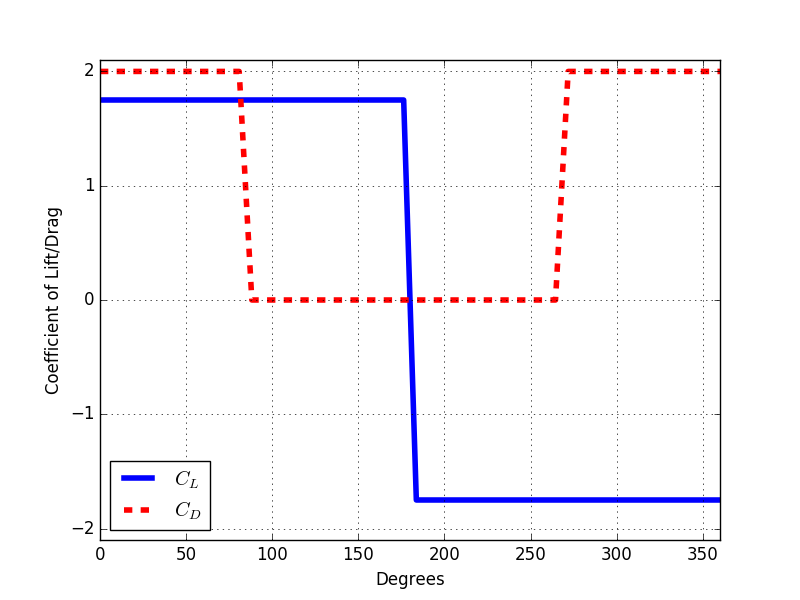
\includegraphics[width = 12 cm]{figs/drags}
    \caption{The idealized drag polars.} 
    \label{drags}
  \end{center}
\end{figure}


\newpage
\section{Questions}

\begin{itemize}
 \item Does this need regularization to ensure well-posedness?
 \item Boundary conditions are periodic
 \item What about supporting twist? (e.g. $\beta = \beta(r)$)
 \item Can we constrain $C_L, C_D$?
 \item Is this just linear programming?
\end{itemize}
Betz limit is 16/27
\end{document}
